\documentclass[14pt,aspectratio=169]{beamer}

\usepackage{pgfpages}
\usepackage{fancyvrb}

\usepackage{tikz}
\usepackage{pgfplots}

\usepackage{minted}
\usemintedstyle{tango}

\usepackage{graphicx}

\usetheme{auriga}
\usecolortheme{auriga}

\setbeamercolor{background canvas}{bg=lightgray}

% define some colors for a consistent theme across slides

\definecolor{red}{RGB}{181, 23, 0}
\definecolor{blue}{RGB}{0, 118, 186}
\definecolor{gray}{RGB}{146, 146, 146}

\title{Web Development: \\ Advanced JavaScript Programming}

\author{{\bf Gregory M. Kapfhammer}}

\institute[shortinst]{{\bf Department of Computer Science, Allegheny College}}

\begin{document}

{
  \setbeamercolor{page number in head/foot}{fg=background canvas.bg}
  \begin{frame}
    \titlepage
  \end{frame}
}

% Slide
%
\begin{frame}{Technical Question}
  %
  \hspace*{.15in}
  %
  \begin{minipage}{5in}
    %
    \vspace*{.5in}
    %
    \begin{center}
      %
      {\large How can I use JavaScript to access the document object model
        (DOM) of a web page to perform page manipulation and to enhance a
      person's interaction with the page?}
      %
    \end{center}
    %
  \end{minipage}
  %
  \vspace{1ex}
  %
  \begin{center}
    %
    \small Let's learn how to use JavaScript to change the layout, content, and
    behavior of a web site! We will explore how to use JavaScript to, for
    instance, manipulate the DOM and verify the content in a web form. Make
    sure to review all previous content about HTML, CSS, and JavaScript! \\
    %
  \end{center}
  %
\end{frame}

% Slide
%
\begin{frame}{The Document Object Model of a Web Page}
  %
  \begin{itemize}
    %
    \item {\bf Document Object Model}: ``Platform- and language-neutral interface
      that will allow programs and scripts to dynamically access and update the
      content, structure, and style of documents.'' Let's explore what this
      means!
      %
      \vspace*{-.15in}
      %
    \item What is the meaning of the W3C definition of the DOM?
      %
      \begin{itemize}
        %
        \item In this case, the ``document'' is the web page!
          %
        \item You can modify the DOM with JavaScript, Java, or Python
          %
        \item You can access the DOM when the browser renders the page
          %
        \item Programs that manipulate the DOM can change multiple page
          characteristics like content, structure, and style
          %
      \end{itemize}
      %
      \vspace*{-.25in}
      %
    \item The {\bf DOM tree} is the data structure that represents a page
      %
  \end{itemize}
  %
\end{frame}

% Slide
%
\begin{frame}{DOM Manipulation with JavaScript}
  %
  \begin{itemize}
    %
    \item The DOM tree contains nodes that represent the elements inside of the
      web page! These nodes contain data about the elements and are related to
      other nodes.
      %
      \vspace*{-.15in}
      %
    \item Three fundamental types of operations for the DOM:
      %
      \begin{itemize}
        %
        \item {\bf Selection Methods}: Extract content from the DOM
          %
        \item {\bf Manipulation Methods}: Change content in the DOM
          %
        \item {\bf Event Methods}: Respond to events when parsing DOM
          %
        \item For instance, {\tt document.write} is a manipulation method!
          %
      \end{itemize}
      %
      \vspace*{-.25in}
      %
    \item Review Figures 9.1 and 9.2 for examples of a DOM tree. See Table 9.1
      for an overview of characteristics about DOM nodes. Questions about
      the basics of the DOM tree?
      %
  \end{itemize}
  %
\end{frame}

% Slide
%
\begin{frame}[fragile]
  \frametitle{JavaScript Selection of Content by Tag}
  \normalsize
  \begin{minipage}{6in}
    \vspace*{.1in}
    \begin{minted}[mathescape, numbersep=5pt, fontsize=\large]{javascript}
const paragraphs =
    document.querySelectorAll("p");
alert(paragraphs[0].nodeName);
alert(paragraphs[0].nodeType);
alert(paragraphs[0].nodeValue);
alert(paragraphs[0].textContent);
    \end{minted}
  \end{minipage}
  %
  \vspace*{.1in}
  %
  \begin{center}
    The {\tt querySelectorAll} returns all matching tags \\
    In this example {\tt paragraphs[0]} is the first {\tt <p>} \\
    The nodes have properties like {\tt nodeName} and {\tt textContent} \\
  \end{center}
  %
\end{frame}

% Slide
%
\begin{frame}[fragile]
  \frametitle{JavaScript Selection of Content by Identifier}
  \normalsize
  \begin{minipage}{6in}
    \vspace*{.1in}
    \begin{minted}[mathescape, numbersep=5pt, fontsize=\large]{html}
<p id="demo"></p>

<script>
  document.getElementById("demo").
              innerHTML = 5 + 6;
</script>
    \end{minted}
  \end{minipage}
  %
  \vspace*{.1in}
  %
  \begin{center}
    The {\tt getElementById} returns an element with an {\tt id} \\
    Using {\tt innerHTML} let's you modify the generated content \\
    This means that a page's HTML content can now be dynamic! \\
  \end{center}
  %
\end{frame}

% Slide
%
\begin{frame}[fragile]
  \frametitle{Dynamically Changing a Page with JavaScript}
  \normalsize
  \begin{minipage}{6in}
    \vspace*{.2in}
    \begin{minted}[mathescape, numbersep=5pt, fontsize=\large]{html}
<div class="jumbotron">
<h1><em>Hello</em> my name is
    Gregory M. Kapfhammer</h1>
<script>
document.write(randomLead());
</script>
</div>
    \end{minted}
  \end{minipage}
  %
  \vspace*{.1in}
  %
  \begin{center}
    What is the definition of the {\tt randomLead()} function?
  \end{center}
  %
\end{frame}

% Slide
%
\begin{frame}[fragile]
  \frametitle{Defining an Array of Strings in JavaScript}
  \normalsize
  \begin{minipage}{6in}
    \vspace*{.2in}
    \begin{minted}[mathescape, numbersep=5pt, fontsize=\normalsize]{javascript}
var lead = [
'<p class="lead">Oh, and I accent the
 <a href="https://github.com/AVMf/avmf">
    AVMf</a>.</p>',
'<p class="lead">Oh, and I predict with
 <a href="https://github.com/Tada-Project/tada">
    tada</a>.</p>',
];
    \end{minted}
  \end{minipage}
  %
  \vspace*{.1in}
  %
  \begin{center}
    The {\tt lead} variable is an array that contains strings of HTML!
  \end{center}
  %
\end{frame}

% Slide
%
\begin{frame}[fragile]
  \frametitle{Randomly Selecting a String from the Array}
  \normalsize
  \begin{minipage}{6in}
    \vspace*{.2in}
    \begin{minted}[mathescape, numbersep=5pt, fontsize=\large]{html}

<script type="text/javascript">
var lead = [ ... ]

function randomLead() {
   return lead[Math.floor(Math.random()
     * lead.length)];
}
</script>

    \end{minted}
  \end{minipage}
  %
\end{frame}

% Slide
%
\begin{frame}[fragile]
  \frametitle{JavaScript Programs Can Respond to Events}
  \normalsize
  \begin{minipage}{6in}
    \vspace*{.2in}
    \begin{minted}[mathescape, numbersep=5pt, fontsize=\large]{html}
<body onload =
      "window.
      alert('Welcome to my page!');"
      >
    \end{minted}
  \end{minipage}
  %
  \vspace*{.1in}
  %
  \begin{center}
    This JavaScript is inline! \\
    Responds to the page loading event \\
    Creates a message in the browser window \\
    Modifies the user's experience when browsing \\
    Any questions about JavaScript programming? \\
  \end{center}
  %
\end{frame}

% Slide
%
\begin{frame}{Event Types in JavaScript}
  %
  \begin{itemize}
    %
    \item JavaScript programs can respond to a wide array of events related to
      page lifecycle or many types of user interaction
      %
      \vspace*{-.15in}
      %
    \item Overview of JavaScript events, with specific examples:
      %
      \begin{itemize}
        %
        \item {\bf Mouse Events}: was the mouse clicked or moved?
          %
        \item {\bf Keyboard Events}: was a key pressed or released?
          %
        \item {\bf Touch Events}: was the screen touched and how?
          %
        \item {\bf Form Events}: was focused changed or form submitted?
          %
      \end{itemize}
      %
      \vspace*{-.25in}
      %
    \item Event-based programming requires JavaScript to listen for the event
      and then respond when the event occurs
      %
      \vspace*{-.25in}
      %
    \item Not all events are supported by all browsers and devices!
      %
  \end{itemize}
  %
\end{frame}

% Slide
%
\begin{frame}{Using JavaScript for Form Validation}
  %
  \begin{itemize}
    %
    \item JavaScript programs can respond to form movement events as a person
      completes fields in the form
      %
      \vspace*{-.15in}
      %
    \item Strategies for validation a submitted form with JavaScript:
      %
      \begin{itemize}
        %
        \item {\bf Empty Fields}: ensure that all required fields have content
          %
        \item {\bf Number Validation}: ensure that numbers are in range
          %
        \item {\bf Text Validation}: ensure that text is of a required length
          %
        \item {\bf Content Validation}: ensure that content has correct form
          %
      \end{itemize}
      %
      \vspace*{-.25in}
      %
    \item Why should we validate form inputs with JavaScript?
      %
      \vspace*{-.25in}
      %
    \item Different browsers display form validation output in different ways.
      Browsers also vary validation defaults!
      %
  \end{itemize}
  %
\end{frame}

% Slide
%
\begin{frame}{AJAX: Asynchronous JavaScript and XML}
  %
  \begin{itemize}
    %
    \item What are the drawbacks of the HTTP request-response loop? Influence on
      the response time and user perception?
      %
      \vspace*{-.35in}
      %
    \item What if the browser could asynchronously return additional data in the
      form of objects encoded in either JSON or XML? What are the benefits of
      this approach?
      %
      \vspace*{-.15in}
      %
    \item When a person interacts with the page and requests a screen update,
      the JavaScript can consult the JSON or the XML instead of making another
      request to the server!
      %
      \vspace*{-.15in}
      %
    \item What are the overall benefits and drawbacks of AJAX?
      %
  \end{itemize}
  %
\end{frame}

% Slide
%
\begin{frame}{JavaScript Linters Can Find (and Fix) Problems}
  %
  \begin{itemize}
    %
    \item JavaScript programs are complicated and often challenging to
      implement, test, and debug. Any assistants to help?
      %
      \vspace*{-.15in}
      %
    \item {\bf JavaScript linter}: tool to check the source code for both
      syntactical and stylistic correctness. Benefits? Drawbacks?
      %
      \vspace*{-.35in}
      %
    \item Overview of JavaScript linters and their use:
      %
      \begin{itemize}
        %
        \item {\bf Environment}: Web-based tools or integrated into your editor
          %
        \item {\bf JSLint}: One of the earliest linting tools
          %
        \item {\bf JSHint}: Originated from JSLint in 2010
          %
        \item {\bf ESLint}: Extensible linter that can fix problems
          %
      \end{itemize}
      %
      \vspace*{-.25in}
      %
    \item What are the specific trade-offs with these tools?
      %
  \end{itemize}
  %
\end{frame}

% Slide
%
\begin{frame}[fragile]
  \frametitle{Configuring the ESLint JavaScript Linting Tool}
  \normalsize
  \begin{minipage}{6in}
    \vspace*{.2in}
    \begin{minted}[mathescape, numbersep=5pt, fontsize=\normalsize]{javascript}
{
  "extends": "gulp",
  "globals": {
    "expect": true
  },
  "rules": {
    "max-len": [2, {"code": 180,
                    "tabWidth": 4,
                    "ignoreUrls": true}]
  }
}
    \end{minted}
  \end{minipage}
  %
\end{frame}

% Slide
%
\begin{frame}[fragile]
  \frametitle{Configuring the ESLint JavaScript Linting Tool}
  \normalsize
  \begin{minipage}{6in}
    \vspace*{.1in}
    \begin{minted}[mathescape, numbersep=5pt, fontsize=\normalsize]{javascript}
{
  "parser": "babel-eslint",
  "extends": [
    "prettier",
    "prettier/react"
  ],
  "env": {
    "es6": true,
    "node": true,
    "jest": true
  }
}
    \end{minted}
  \end{minipage}
  %
\end{frame}

% Slide
%
\begin{frame}{Using the Prettier Code Formatter for JavaScript}
  %
  \begin{figure}
    \centering
    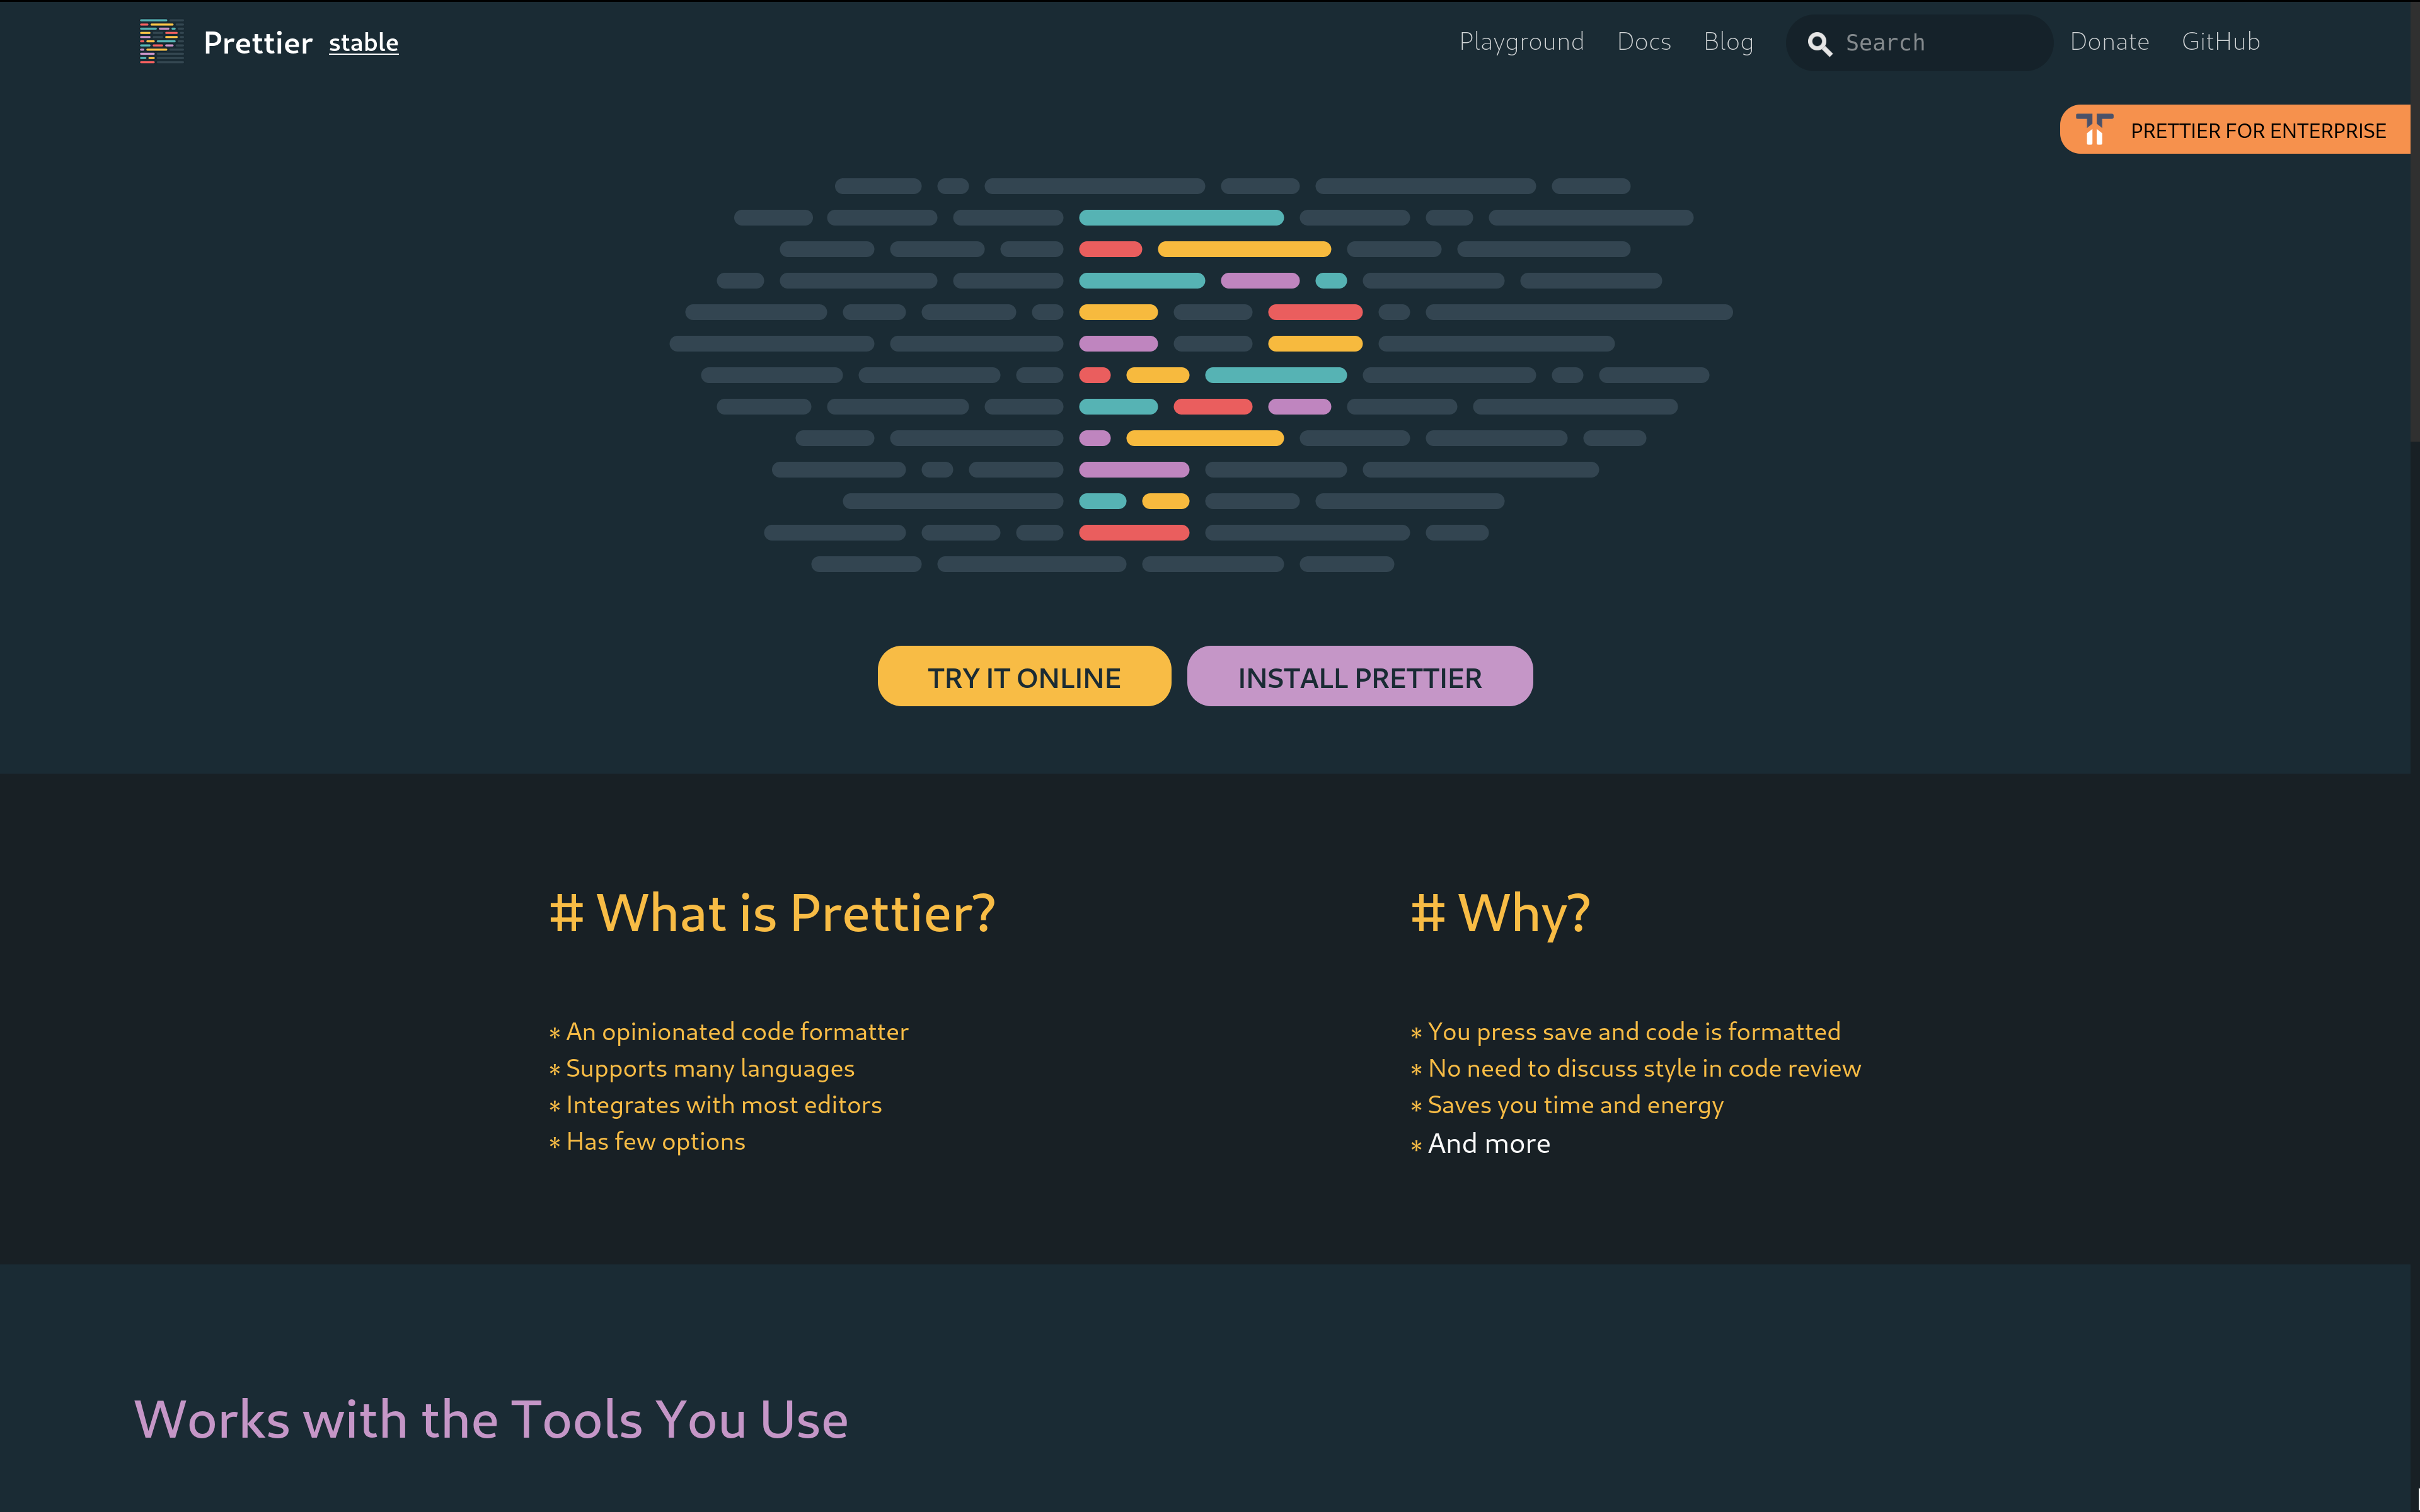
\includegraphics[scale=.080]{images/prettier.png}
    \caption{The figure's caption}
  \end{figure}
  %
\end{frame}

% Slide
%
\begin{frame}{Automated Testing with JavaScript Tools}
  %
  \begin{itemize}
    %
    \item JavaScript programs are complicated and often challenging to
      implement, test, and debug. Any assistants to help?
      %
      \vspace*{-.15in}
      %
    \item {\bf JavaScript testing framework}: tool to run source code and check
      output for correctness.
      %
      \vspace*{-.15in}
      %
    \item Overview of JavaScript testing framework and their use:
      %
      \begin{itemize}
        %
        \item {\bf Environment}: command-line or integrated into your editor
          %
        \item {\bf Jest}: Developed by Facebook and suitable for React
          %
        \item {\bf Mocha}: Supports both NodeJS and browser JavaScript
          %
        \item {\bf Jasmine}: Framework-independent JavaScript testing
          %
      \end{itemize}
      %
      \vspace*{-.25in}
      %
    \item Refer to \url{https://stateofjs.com/} to learn more!
      %
  \end{itemize}
  %
\end{frame}

% Slide
%
\begin{frame}{Explore the State of JavaScript Survey}
  %
  \begin{figure}
    \centering
    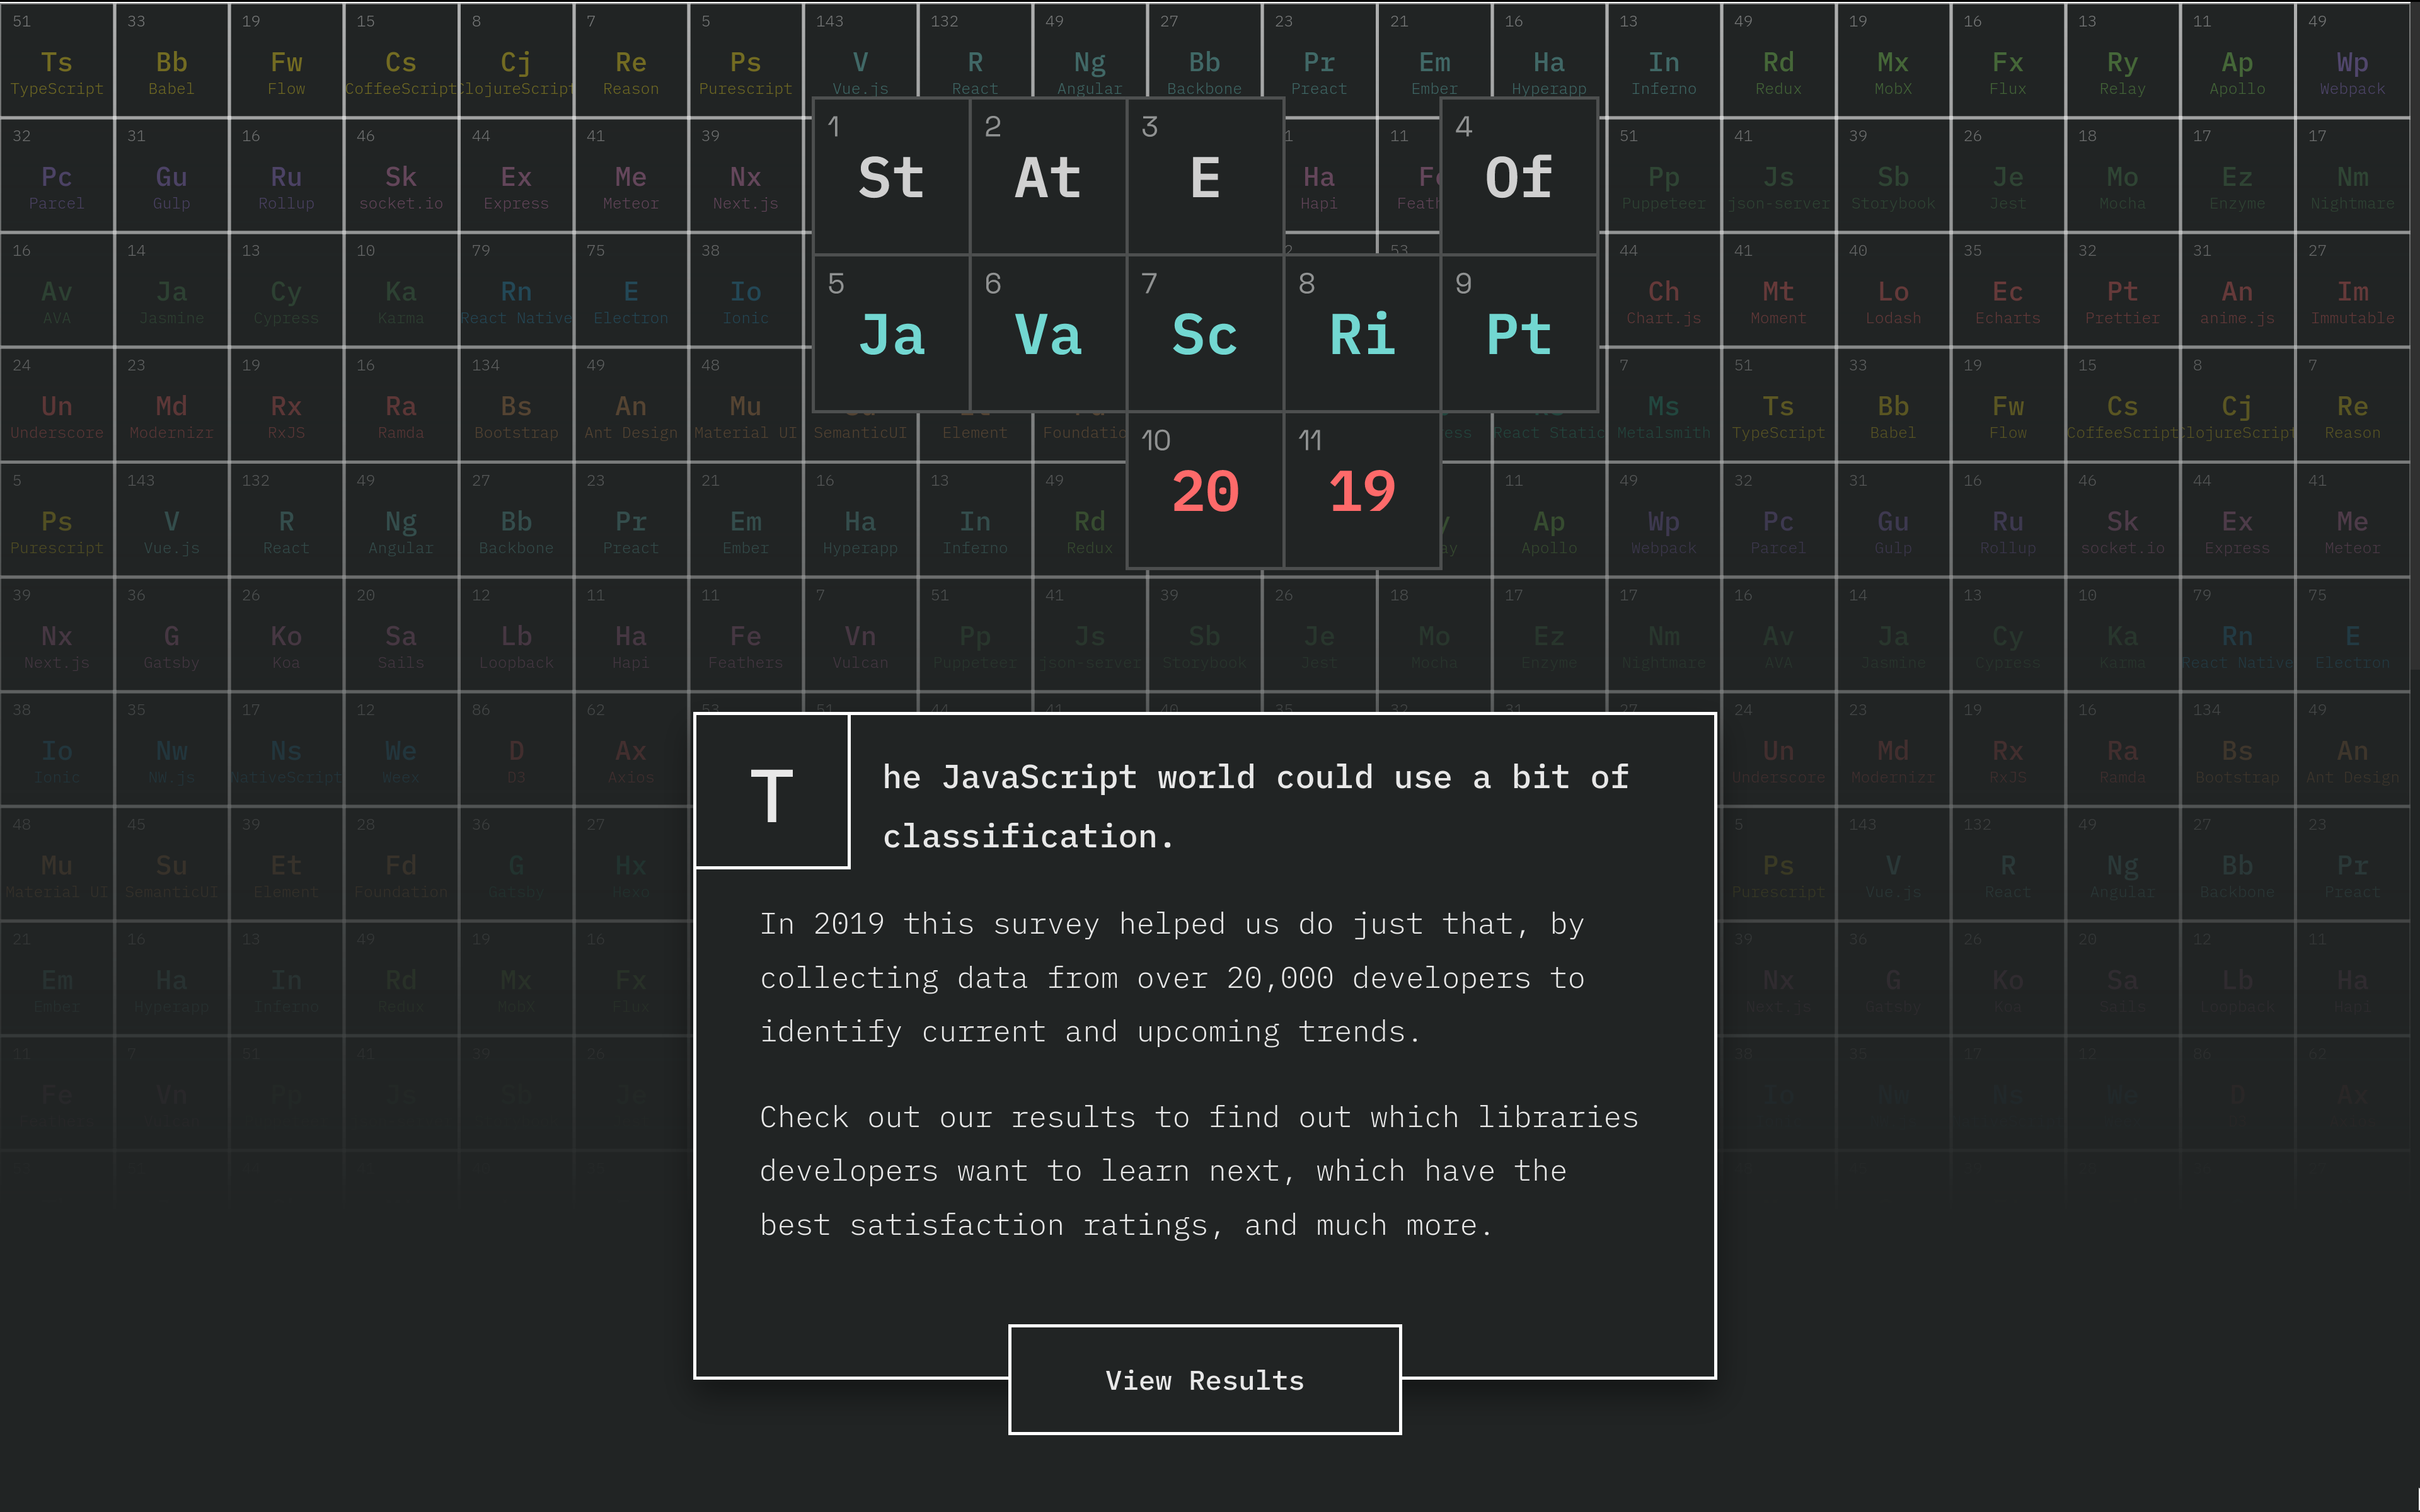
\includegraphics[scale=.080]{images/stateofjs.png}
    \caption{The figure's caption}
  \end{figure}
  %
\end{frame}

% Slide
%
\begin{frame}{Learn More about JavaScript}
  %
  \begin{figure}
    \centering
    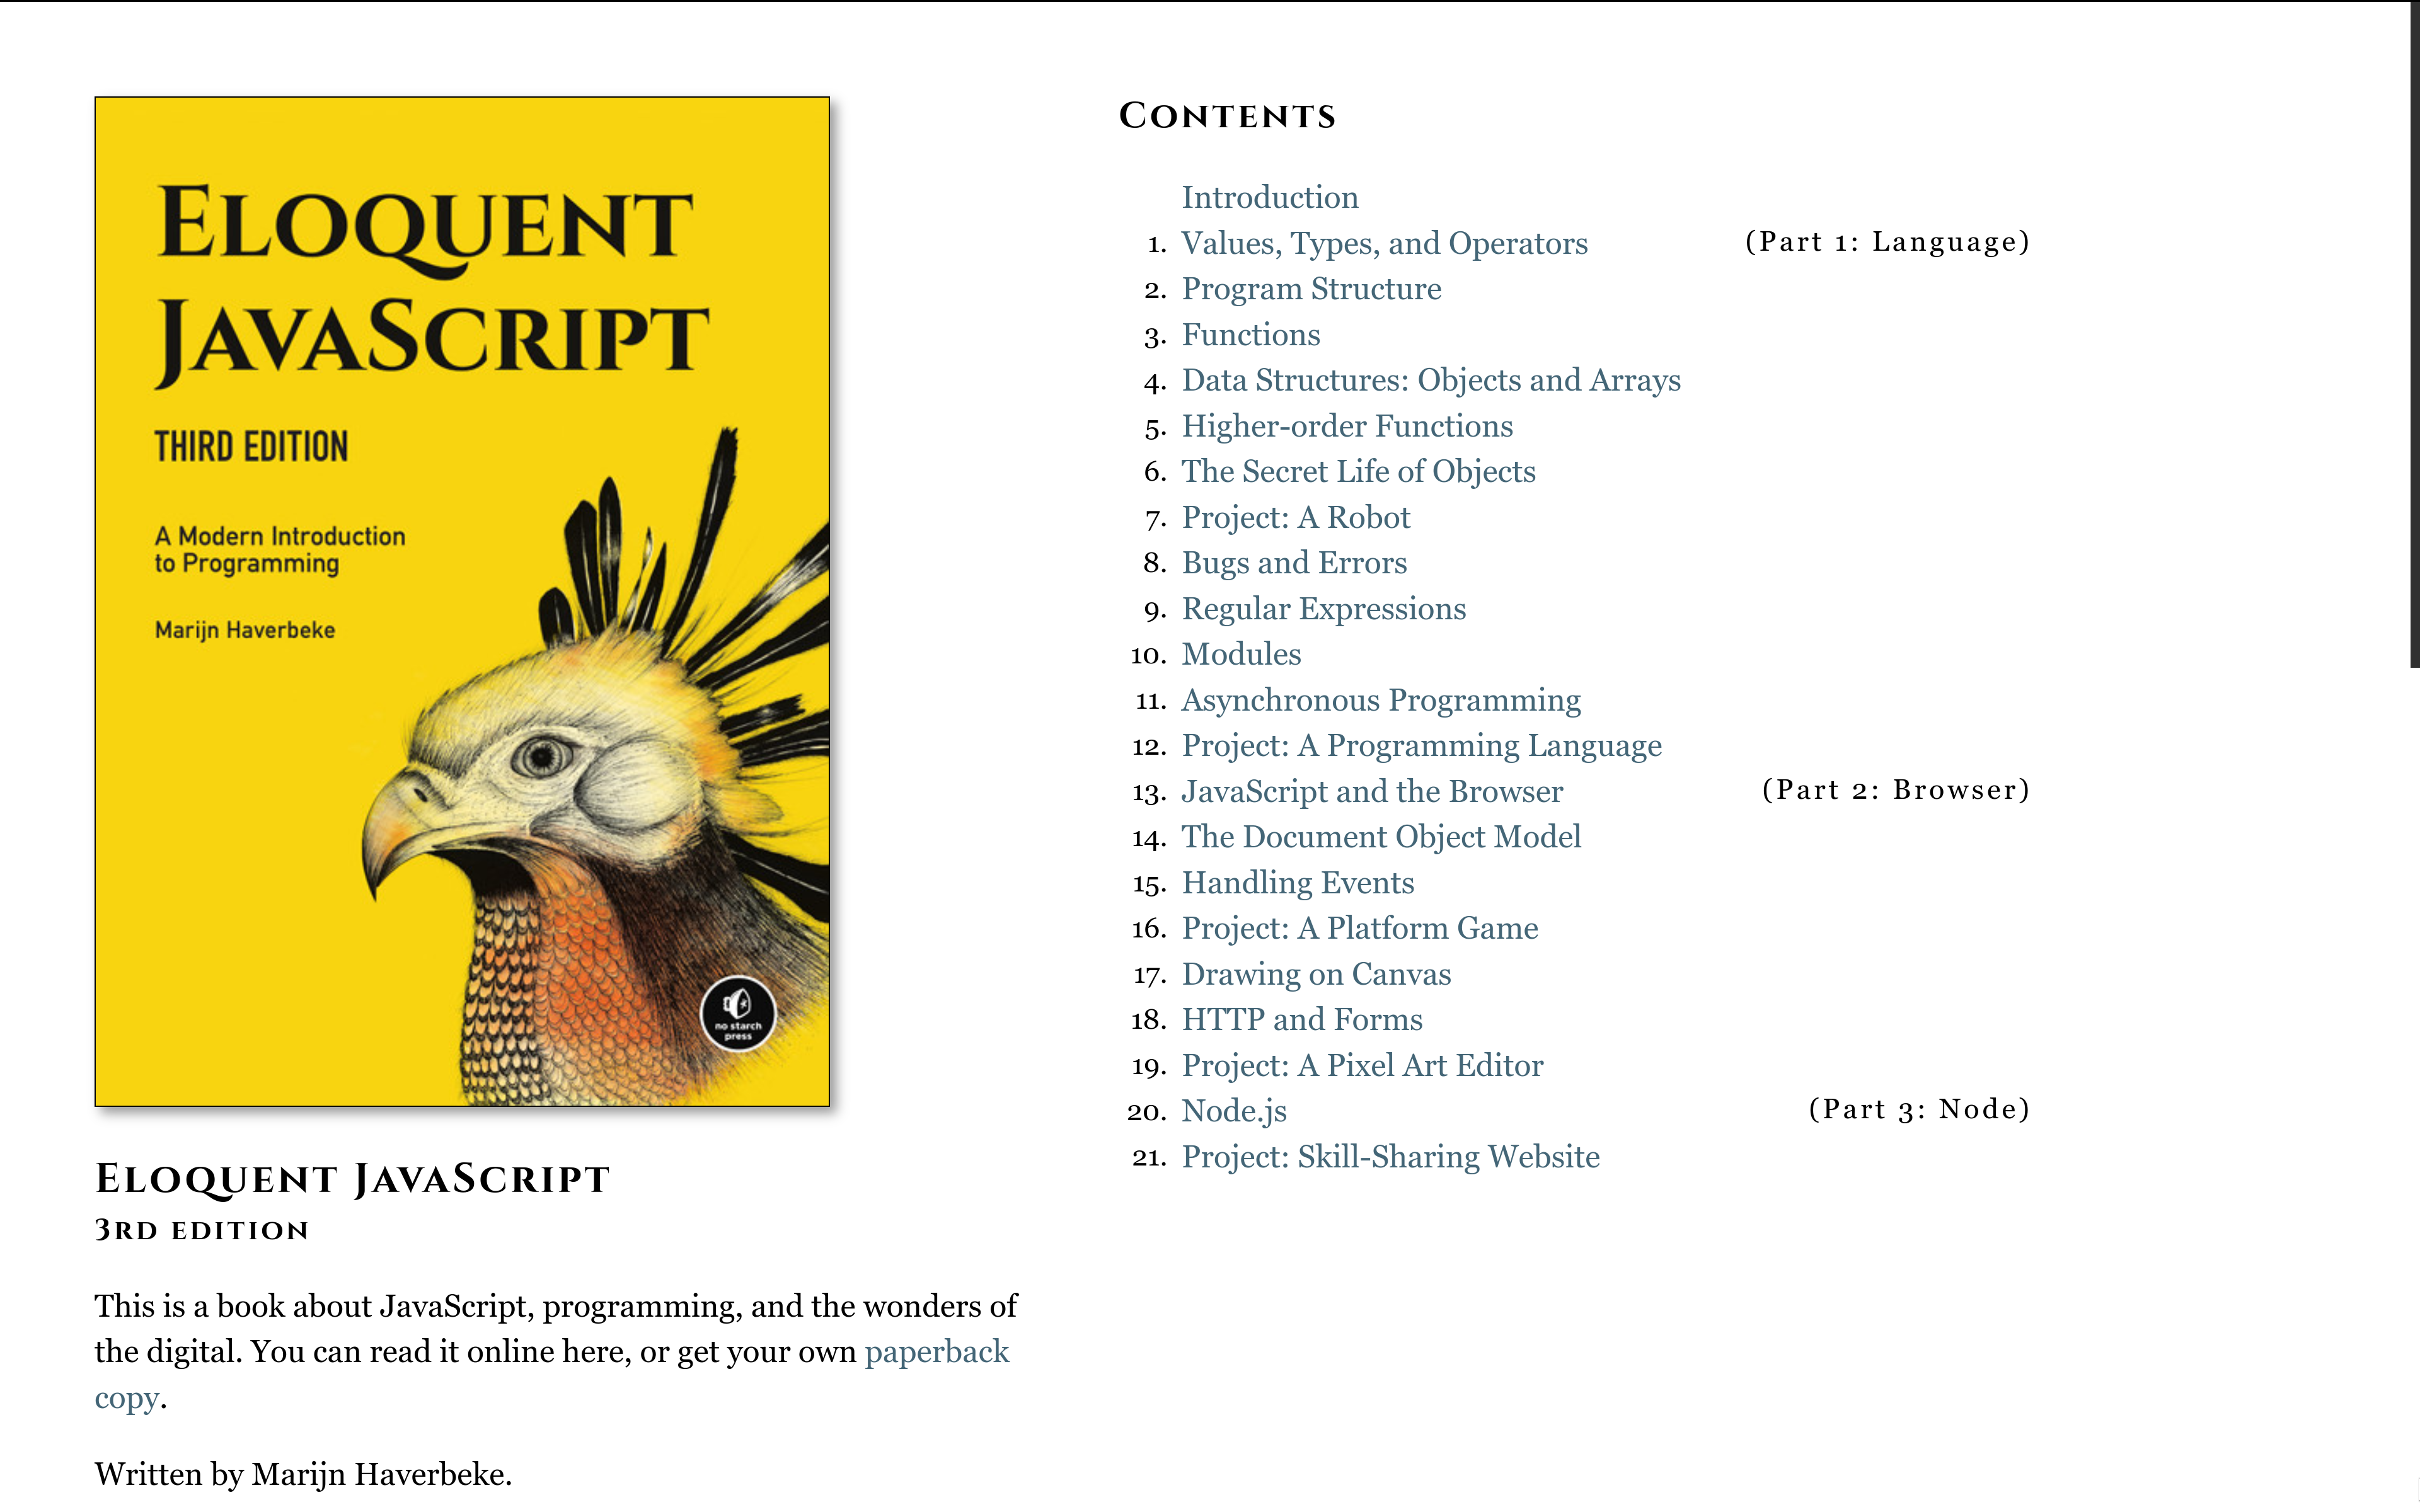
\includegraphics[scale=.080]{images/eloquent-javascript.png}
    \caption{The figure's caption}
  \end{figure}
  %
\end{frame}

% Slide
%
\begin{frame}{Learn What You Don't Know About JavaScript!}
  %
  \begin{figure}
    \centering
    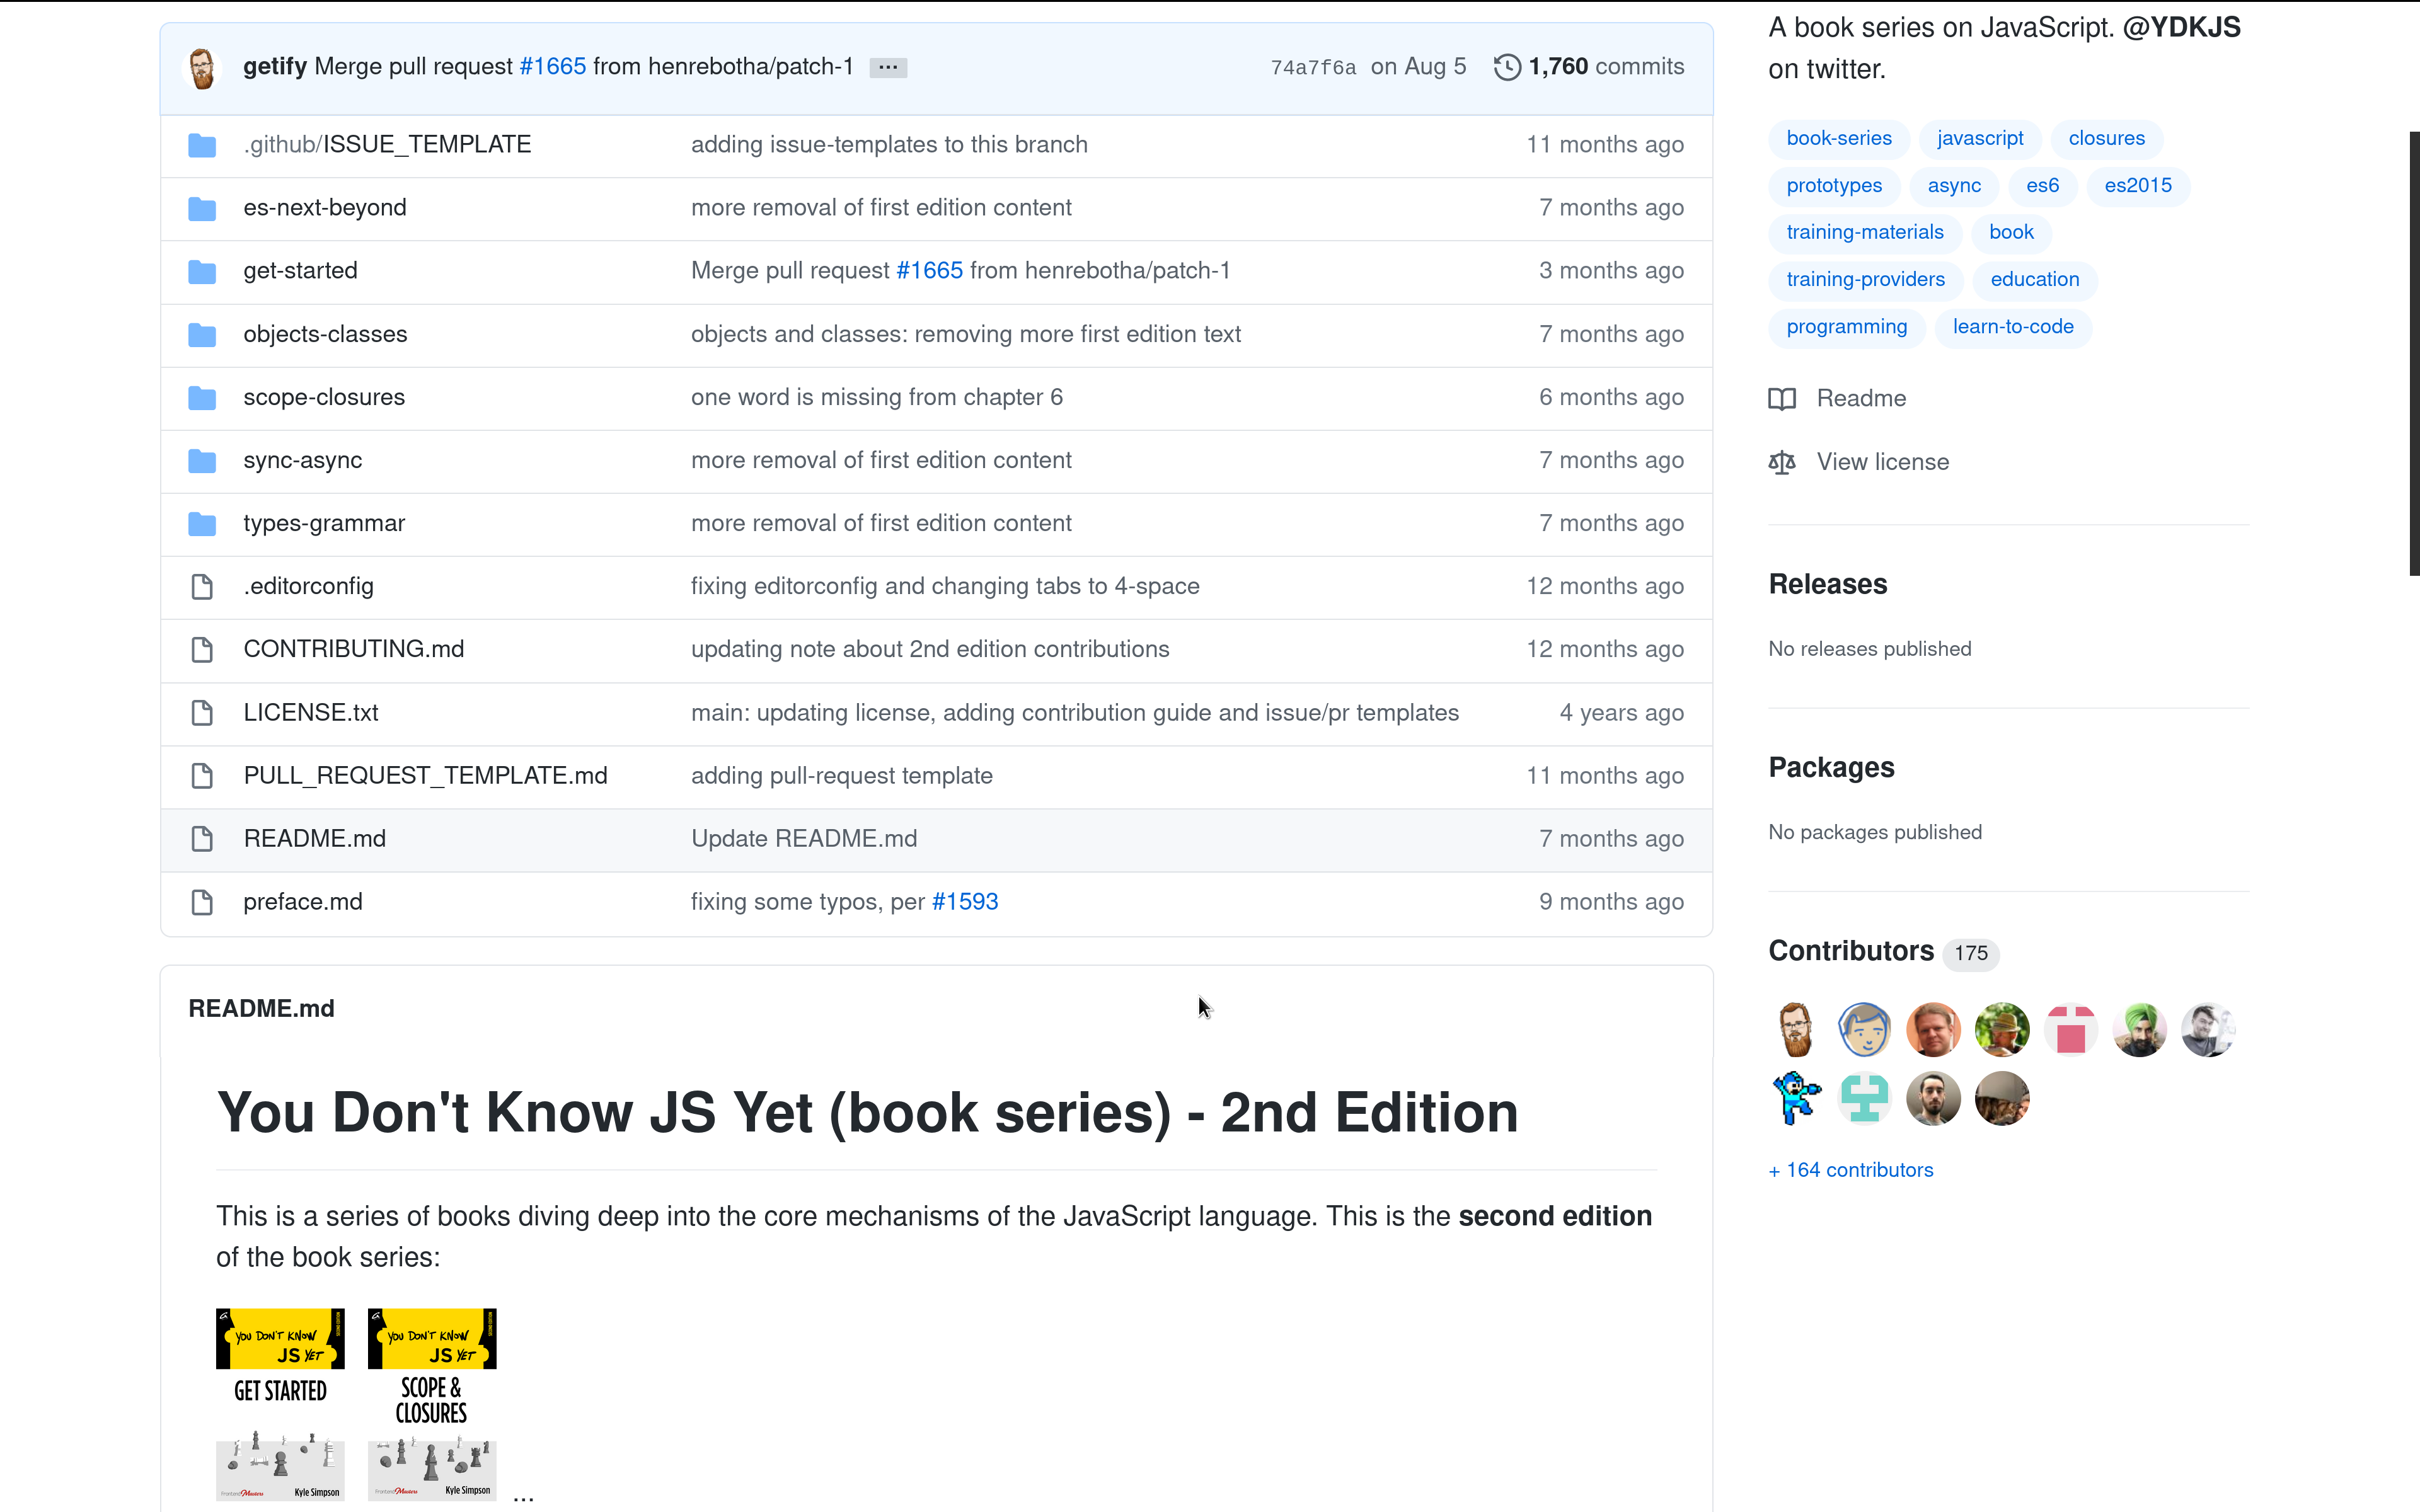
\includegraphics[scale=.080]{images/dont-know-javascript.png}
    \caption{The figure's caption}
  \end{figure}
  %
\end{frame}

\end{document}
